\section{Features and Implementation}

\mkado is implemented in Python
and provides a command-line interface built on Typer.
It accepts codon-aligned FASTA files as input,
requiring no pre-processing or external format conversion.
Sequences are automatically partitioned into ingroup and outgroup sets
by name pattern matching,
supporting both multi-species alignments in a single file
and separate ingroup/outgroup files.
Full documentation, including tutorials and API reference,
is available at \url{https://mkado.readthedocs.io}.

\paragraph{Analysis methods}
\mkado implements three MK test variants.
The \textit{standard} test computes the classical $2 \times 2$ table
of nonsynonymous and synonymous changes
in polymorphism and divergence (Dn, Ds, Pn, Ps),
with significance assessed by Fisher's exact test.
Summary statistics include the neutrality index \citep{rand1996},
$\alpha$ \citep{smith2002},
and the Direction of Selection statistic
\citep[DoS;][]{stoletzki2011}.
The \textit{polarized} test uses a second outgroup
to infer the ancestral state at each fixed difference,
assigning divergence to the ingroup or outgroup lineage
for lineage-specific inference.
The \textit{asymptotic} test bins polymorphisms
by derived allele frequency (DAF),
computes $\alpha$ within each bin,
and fits an exponential model $\alpha(x) = a + b e^{-cx}$
to extrapolate the asymptotic $\alpha$ at $x = 1$,
correcting for the contribution of weakly deleterious variants
\citep{messer2013}.
Confidence intervals are obtained by bootstrap resampling.

\paragraph{Codon change classification}
When comparing codons that differ at multiple positions,
the assignment of changes as synonymous or nonsynonymous
is not straightforward
because the order of substitutions is unknown.
\mkado pre-computes all shortest mutational paths
between every pair of codons
and weights the synonymous and nonsynonymous contributions
equally across paths,
following the approach of \citet{nei1986}.

\paragraph{Batch processing and parallelism}
The \texttt{batch} command processes directories of alignment files
in parallel using Python's multiprocessing facilities
with configurable worker counts.
Benjamini-Hochberg adjusted $p$-values
are computed automatically across all genes.
To evaluate scaling performance,
we benchmarked \mkado on 12,437 human protein-coding genes
aligned with chimpanzee and orangutan orthologs
from OrthoMaM \citep{orthomam2024},
with polymorphism data from 178 Yoruba individuals
in the 1000 Genomes Project \citep{1000genomes2015}.
Processing all genes with 128 worker threads
completed in 28 seconds
(50$\times$ speedup over single-threaded execution),
with near-linear scaling up to 32 threads
and sustained efficiency at higher thread counts
(\cref{fig:benchmark}).

\paragraph{Visualization}
\mkado generates publication-ready plots
directly from the command line.
Volcano plots display $-\log_{10}(\text{NI})$
against $-\log_{10}(p)$ for each gene,
with Bonferroni and nominal significance thresholds
(\cref{fig:volcano}).
The asymptotic test produces $\alpha(x)$ curves
showing the fitted model and bootstrap confidence intervals.

\begin{figure}[!t]
  \centering
  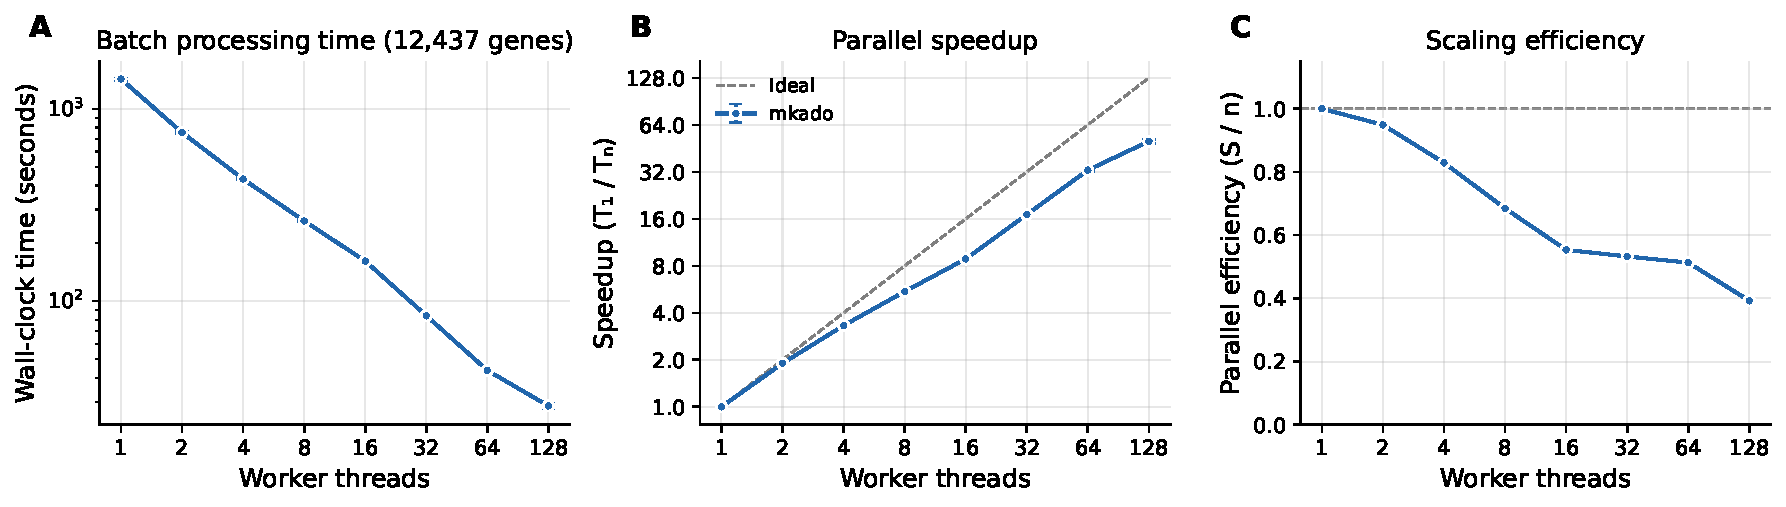
\includegraphics[width=\columnwidth]{figures/mkado_benchmark.pdf}
  \caption{Parallel scaling of \mkado batch processing on 12,437 human
    protein-coding genes. (\textbf{A})~Wall-clock time versus worker threads.
    (\textbf{B})~Speedup relative to single-threaded execution, with ideal
    linear scaling shown as a dashed line. (\textbf{C})~Parallel efficiency
    (speedup divided by thread count).}
  \label{fig:benchmark}
\end{figure}

\begin{figure}[!t]
  \centering
  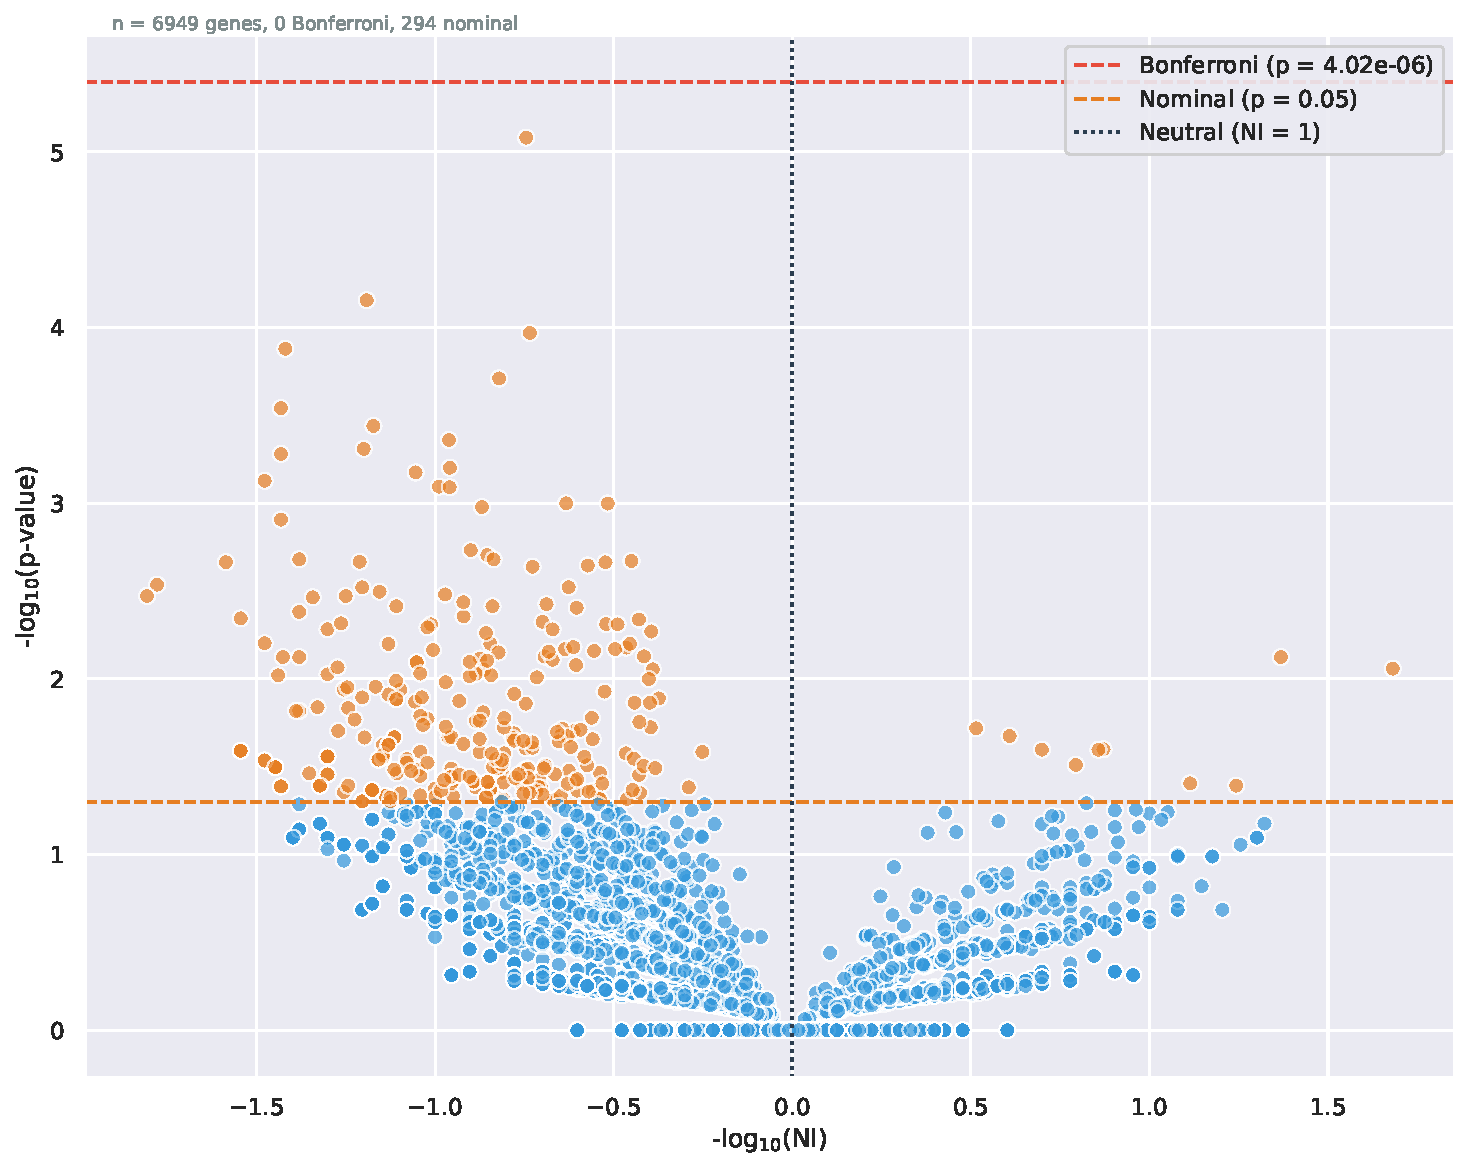
\includegraphics[width=0.85\columnwidth]{figures/mk_volcano_pan.pdf}
  \caption{Volcano plot from standard MK tests on 12,437 genes using
    \textit{Pan troglodytes} as the outgroup.
    Orange points are nominally significant ($p < 0.05$);
    dashed lines indicate Bonferroni and nominal thresholds.
    The leftward shift of the cloud (NI $> 1$) reflects the
    well-known excess of weakly deleterious nonsynonymous polymorphism
    in humans.}
  \label{fig:volcano}
\end{figure}
